\documentclass{article}
\usepackage[utf8]{inputenc}
\usepackage{graphicx}
\usepackage{amsmath}
\usepackage{subfig}
\usepackage{titlesec}
\usepackage{hyperref}
\graphicspath{ {./images/} }
\hypersetup{
    colorlinks=true,
    linkcolor=blue,
    filecolor=magenta,
    urlcolor=cyan,
    pdftitle={Overleaf Example},
    pdfpagemode=FullScreen,
    }

\title{Code Theorie Project\\\\ University Antwerp}
\author{Cédric Leclercq, Elias Dams, Robbe Nooyens}
\date{December 2022}

\begin{document}

\maketitle

\tableofcontents

\newpage

\section{vigenerePlus}
\subsection{About}
ViginairePlus is a chipher in which first viginaire and then single column transposition is applied. Two different keywords are used in this process.\\
\\
I found it very difficult to find a suitable approach. Vigenère's weakness is Kasiski's test and coincidence index. However, if you put column transposition on top of Vigenère, that weakness is gone. The text is now shuffled and you can't search for digraphs/trigraphs because they give the wrong key length pattern. Nor can you solve for Columnar Transposition. Because the resulting text is still encrypted with vigenere.\\
\\
If we want to brute force (assuming we both have keys with a maximum length of 10). we have to go through all the permutations. That makes a total of 16304741395569 possibilities. This is just not possible\\
\\
$\sum_{i=1}^{10} i! \cdot \sum_{j=1}^{10} j! = 16304741395569$\\
\subsection{Single-column transposition}
We must first solve the column transposition. We do this by going over all possible permutations of maximum length 10 (otherwise it takes a long time) and making a selection. So we will have to identify how hard a transposed cyphertext resembles a vigenere chipher. As mentioned earlier, a coincidence index will not say much. Because only the order of the letters changes.\\
\\
What we can do however is run a kasiski test. Kasiski suggested looking for repeated fragments in the ciphertext and making a list of the distances separating the repetitions. Then the length of the keyword is likely to divide many of these distances. With a non vigenere text this test will not be of much use and all key lengths are equally possible. However, with a vigenere text there will often be an outlier of a possible key length. If there is such an outlier I write it to a file. So after a run of the first part of my algorithm we have a file consisting of all the vigenere ciphertexts with a possible vigenere key length. So we have reduced the number of possibilities considerably.\\
\\
(if the outlier has length smaller than 4 then I manually remove it, because this is an unrealistically small key.)
\newpage
\subsection{Vigenère}
Now we only have a list of vigenere encrypted messages and their possible key lenght(s). To guess the key we are going to use the \href{http://practicalcryptography.com/media/cryptanalysis/files/english_bigrams_1.txt}{bigrams}, and their appearance in the english language. I will explain the algorithm using an example.\\
\\
Plaintext: Codetheorieproject\\
Ciphertext: Msboxfospsinbshogr\\
Key: KEY\\
\\
We loop over the text and take the doubles that are 3 positions apart (keylenght). The doubles we are going to use to determine the first letter of the key are Ms, ox, os, si, bs and og.\\
\\
\hspace*{-0.5in}
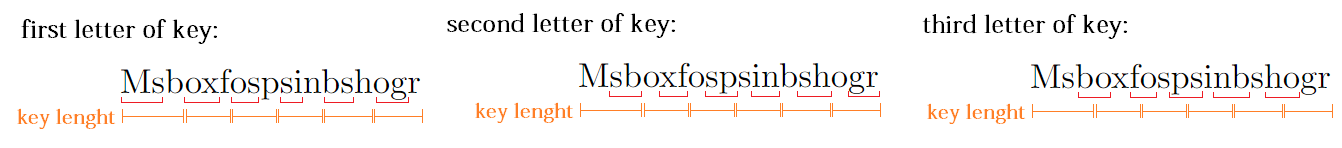
\includegraphics[scale=0.60]{image1.png}
\\
Then we will calculate the entropy value ( from the table) of these doubles and all their possible shifts. At the end we look at the lowest entrpy value. We look at the shifts. Since our key is "KEY", +11 in the example will have the lowest entropy. The 11th letter is K. This is how we determined the first letter of the key. We repeat this for each letter of the key.\\
\hspace*{-0.5in}
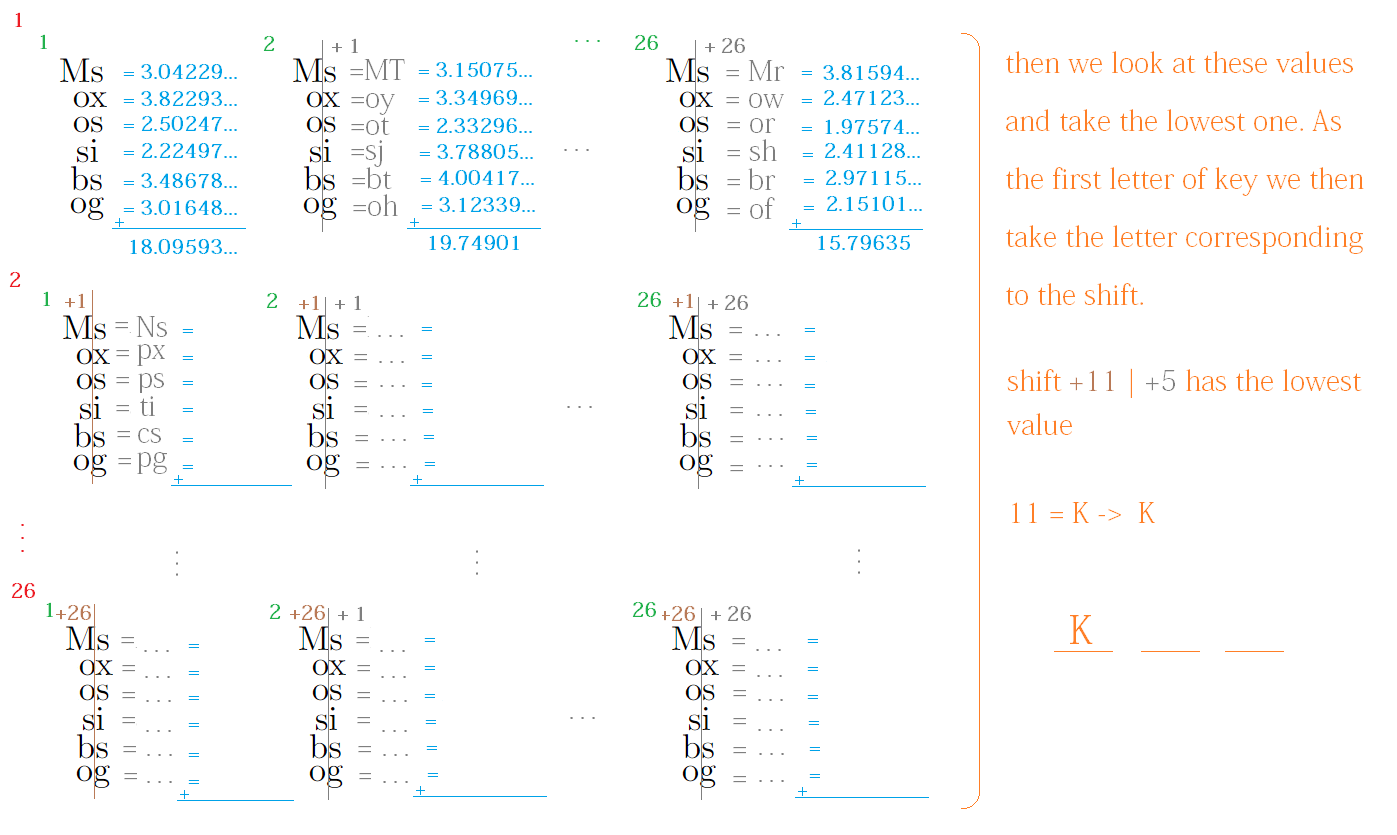
\includegraphics[scale=0.60]{image2.png}
\\
Then we take the final key and use it to find the plaintext. Then calculate the entropy of the resulting text. If it looks like English, we write it to a file. \\
(I noted that this doesn't always work for small texes, but the texes we got were large enough to find a correct solution each time).

\section{playfair}
\section{adfgvx}
\section{enigma}

\end{document}